\input vv285mla
\def\k{\kappa}
\def\r{\gamma}
\def\dr{\gamma'(t)}
\def\ddr{\gamma''(t)}
\def\dddr{\gamma'''(t)}
\def\ctt{\cos t}
\def\stt{\sin t}
\begin{document}
\titlehm{7}
\ep{1}{
\item[i)]
	\def\k{\kappa}
	The rate of change in tangent vector with respect to 
	curve length is proportional to the normal vector, with
	the coefficient curvature.\\
	This follows from definition:
	\eq{
	\kappa N=\left\|\ff{dT}{ds}\right\|
	\times\ff{dT}{ds}\Big/\left\|\ff{dT}{ds}\right\|
	=\ff{dT}{ds}
	}
\item[ii)]
	\def\cp{\cos\varphi}
	\def\sp{\sin\varphi}
	\def\p{\varphi}
	This follows from geometry:
	\eq{
	\cp=\dotp{T}{e_1}\implies -\sp\,\ff{d\p}{ds}=
	\dotp{\ff{dT}{ds}}{e_1}
	}
	now we assume that $\p\neq0$ since it's smooth, we have:
	\eq{
	\left\|\ff{d\p}{ds}\right\|&=\dotp{\ff{dT}{ds}/\sp}{e_1}\\
	&\quad=\left|\dotp{\k \ff{N}{\sp}}{e_1}\right|\\
	&\quad=\ff{\k}{|\sp|}|\dotp{N}{e_1}|\\
	&\quad=\k\ff{1}{|\sp|}\|N\||\cos(\p+\pi/2)|\\
	&\quad=\k
	}
	The last line follows from the fact that the normal vector 
	forms an angle of $\p+\pi/2$ of $e_1$ if the tangent forms 
	an angle of $\p$ of $e_1$.
\item[iii)]
	First its norm:
	\eq{
	\nn{B}=\nn{T}\nn{N}\sin\ff{\pi}{2}=1
	}
	and by product rule:
	\eq{
	\dd{B}{s}=\dd{T}{s}\times N+T\times\dd{N}{s}=T\times\dd{N}{s}
	}
	since $dT/ds$ and $N$ are parallel. Then:
	\eq{
	\dotp {B}{\dd{B}{s}}&=\dotp
	{\left( T\times N \right)}
	{\left( T\times \dd{N}{s} \right)}\\
	&=-\dotp{N}{T\times\left(T\times\dd{N}{s}  \right)}\\
	&=-\dotp{N}{\dd{N}s}\\
	&=0
	}
	where we use the fact that 
	\eq{
	0=\dd{}{s}\dotp{N}{N}=2\dotp{N}{\dd{N}{s}}
	}
	thus
	\eq{
	\dd{B}{s}\perp B
	}
	and another relation
	\eq{
	\dd{B}{s}\perp T
	}
	is trivial since $T\times dN/ds$ is perpendicular to $T$ by
	the definition of cross product.\\
	Then, we conclude that one can write
	\eq{
	\dd{B}{s}=-\tau(s)N
	}
\item[iv)]
	By the sprite of previous exercise $T$, $N$ and $B$ forms
	a right hand system, and we rewrite it as:
	\eq{
	N=B\times T
	}
	differentiate it:
	\eq{
	\dd{N}{s}&= \dd{B}{s}\times T+B\times\dd{T}{s}\\
	&= -\tau N\times T+\k B\times N\\
	&=-\k T+\tau B
	}
	where again we use the results of the previous exercises
	and the right hand relation.
}
\ep{2}{
\def\k{\kappa}
\def\r{\gamma}
\def\dr{\gamma'(t)}
\def\ddr{\gamma''(t)}
\def\dddr{\gamma'''(t)}
\item[]
	We summary the result of the previous exercise by chain rule:
	\eq{
	\dd{}{t}\mm{T\\N\\B}=
	\|\dr\|\mm{&\k&\\-\k&&\tau\\&-\tau&}
	\mm{T\\N\\B}
	}
	this is due to the fact that:
	\eq{
	\dd{}{t}\mm{T\\N\\B}=\dd{}{s}\mm{T\\N\\B}\dd{s}{t}=
	\dd{}{s}\mm{T\\N\\B}\|\dr\|
	}
	and the convention by definition:
	\eq{
	l'=\|\dr\|
	}
	therefore, by definition:
	\eq{
	\ddr&=\dd{}{t}\dr=\dd{}{t}\|\dr\|T=\dd{}{t}l'T\\
	&=l''T+l'\dd{T}{t}=l''T+\k(l')^2N
	}
	and the third derivative:
	\eq{
	\dddr&=\dd{}{t}\left(l''T+\k(l')^2T  \right)\\
	&\quad=l'''T+l''\dd{T}{t}+k'(l')^2N
	+2\k l'l''N+\k(l')^2\dd{N}{t}\\
	&\quad=(l'''-\k^2(l')^3)T
	+\left( 3\k l'l''+k'(l')^2 \right)N
	+\k\tau(l')^3B
	}
	and finally 
	\eq{
	\dr\times\ddr&=lT\times\left(l''T+\k(l')^2N  \right)\\
	&=\k(l')^3B
	}
	Now it remains to verify:
	\eq{
	\dotp{\r'\times\r''}{\r'''}=\k^2(l')^6\tau=\|\r'\times\r''\|
	\tau\\
	\implies\tau=\ff{\dotp{\r'\times\r''}{\r'''}}
	{\|\r'\times\r''\|^2}=\ff{\det\left( \r',\r'',\r''' \right)}
	{\|\r'\times\r''\|^2}
	}
}
\es{3}{
\item[i)]
	\eq{
	T=\ff{1}{\sq{r^2+h^2}}\mm{-r\stt\\ r\ctt\\ h}\quad
	N=\mm{-\ctt\\ -\stt\\ 0}\quad
	B=T\times N=\ff{1}{\sq{r^2+h^2}}\mm{h\stt\\ -h\ctt\\ r}
	}
\item[ii)]
	We use the formula in the lecture:
	\eq{
	\k=\ff{\|\dr\times\ddr\|}{\|\dr\|^3}=
	\left\|\mm{-r\stt\\ r\ctt\\ h}\times\mm{-r\ctt\\ -r\stt\\ 0}\right\|\Big/
	\left(\sq{r^2+h^2}\right)^3=\ff{r}{r^2+h^2}
	}
	and the formula in the previous exercise:
	\eq{
	\tau=\ff{\dotp{\r'\times\r''}{\r'''}}{\|\r'\times\r''\|^2}=\ff{h}{r^2+h^2}
	}
\item[iii)]
	Straight from the definition:
	\eq{
	m(t)=\r(t)\times \mm{0\\0\\-F}=\mm{-Fr\stt\\Fr\ctt\\0}
	}
	and by projection:
	\eq{
	&m_T=\dotp{m(t)}{T}T=\ff{Fr^2}{R}T\\
	&m_B=\dotp{m(t)}{B}B=-\ff{Frh}{R}B
	}
\item[iv)]
	Notice from definition
	\eq{
	&H=2\pi nh\\
	&r^2=\left(\ff{1}{2\pi n}\right)^2\left(L^2-(2\pi n h)^2\right)
	=\left(\ff{L}{2\pi n}\right)^2-h^2
	}
	and therefore
	\eq{
	&\k=2\pi n\ff{1}{L}\sq{1-\left(\ff{H}{L}\right)^2}\\
	&\tau=2\pi n\ff{H}{L^2}
	}
	Introducing the pitch angle:
	\eq{
	&\k=2\pi n\ff{\cos\alpha}{L}\\
	&\tau=2\pi n\ff{\sin\alpha}{L}
	}
\item[v)] 
	Simply plug in the relation in iv):
	\eq{
	(H-H(F))\cdot GJ=\ff{rL^2}{2\pi n}F
	}
	and dividing by $H-H(F)$, set $F\to 0$, notice one side is independent of $F$:
	\eq{
	c=\ff{2\pi n \cdot GJ}{rL^2}
	}
\item[vi)]
	Plug in the numbers:
	\eq{
	&L_f= 263\,{\rm cm}&  &L_r=297\,{\rm cm}\\
	&c_f=1.47\times 10^2& &c_f=1.90\times 10^2\\
	&H-H_f=2.44{\rm cm}& &H-H_r=10.89{\rm cm}
	}
}
\es{4}{
\item[i)]
	\eq{
	T=\ff{1}{3}\mm{2\\2\\1}\quad
	N=\ff{1}{3}\mm{-1\\2\\-2}\quad
	B=\ff{1}{3}\mm{2\\-1\\-2}\quad
	\k=\ff{2}{9}\quad
	\tau=\ff{2}{9}
	}
\item[i)]
	\eq{
	T=\ff{1}{\sq{3}}\mm{1\\1\\1}\quad
	N=\ff{1}{\sq{2}}\mm{0\\1\\-1}\quad
	B=\ff{1}{\sq{6}}\mm{-2\\1\\1}\quad
	\k=\ff{\sq{2}}{3}\quad
	\tau=-\ff{1}{3}
	}
}
\es{5}{
\nopagebreak
\pgfplotsset{compat=1.8}
\item[i)]
	$r=\cos(2\theta)$:
	\begin{center}
		\begin{tikzpicture} 
			\begin{polaraxis}[
				 axis equal, 
			 	minor tick num=1, 
			 	] 
		 	\addplot
			 	[blue,
				 domain=0:360,
				 samples=200, 
				 smooth,
				 data cs=polar]
				 (x,{cos(2*x)});
			\end{polaraxis}
		 \end{tikzpicture}
	 \end{center}
	 \vskip 2em
\item[ii)]
	$r=\cos(3\theta)$:
	 \begin{center}
		\begin{tikzpicture} 
			\begin{polaraxis}[		
				 axis equal, 
			 	minor tick num=1, 
			 	] 
		 	\addplot
			 	[blue,
				 domain=0:360,
				 samples=200, 
				 smooth,
				 data cs=polar]
				 (x,{cos(3*x)});
			\end{polaraxis}
		 \end{tikzpicture}
	 \end{center}
	  \vskip 2em
\item[iii)]
	$r=|\cos(2\theta)|$:
	 \begin{center}
		\begin{tikzpicture} 
			\begin{polaraxis}[
				 axis equal, 
			 	minor tick num=1, 
			 	] 
		 	\addplot
			 	[blue,
				 domain=0:360,
				 samples=200, 
				 smooth,
				 data cs=polar]
				 (x,{abs(cos(2*x))});
			\end{polaraxis}
		 \end{tikzpicture}
	 \end{center}
	  \vskip 2em
\item[iv)]
	$r=|\cos(3\theta)|$:
	 \begin{center}
		\begin{tikzpicture} 
			\begin{polaraxis}[
				 axis equal, 
			 	minor tick num=1, 
			 	] 
		 	\addplot
			 	[blue,
				 domain=0:360,
				 samples=200, 
				 smooth,
				 data cs=polar]
				 (x,{abs(cos(3*x))});
			\end{polaraxis}
		 \end{tikzpicture}
	 \end{center}
}
\es{6}{
\item[]
	We proceed as in the lecture:
	\eq{
	l=a\int_0^{2\pi}\sq{(1-\cos t)^2+\sin^2 t}\,dt=2a\int_0^{2\pi}\sin\ff{t}{2}\,dt=8a
	}	
}
\es{7}{
\item[i)]
	Notice that if $t$ satisfy the curve, we have:
	\eq{
	\left(\ff{3t}{1+t^3},\quad\ff{3t^2}{1+t^3}\right)=
	\left(\ff{3\ff{1}{t^2}}{1+\ff{1}{t^3}},\quad\ff{3\ff{1}{t}}{1+\ff{1}{t^3}}\right)
	}
	thereby $(a,b)$ being on the curve induces $(b,a)$ to be on the curve with a different parameter $1/t$. And when $t=0$ the symmtry is trivial: $(0,0)$.\\
	Notice the only intersection to the line $y=x$ is $(0,0)$.
\item[ii)]
	\eq{
	\dr=\left(\ff{3(1-2t^3)}{(1+t^3)^2},\quad\ff{3(2t-t^4)}{(1+t^3)^2}\right)
	}
	horizontal implies
	\eq{
	&\quad t=0\quad{\rm or}\quad t=2^{1/3}\\
	&\implies\left(2^{1/3},\quad2^{2/3}\right)
	}
	since $(0,0)$ there the tangent line is undefined.
	And vertical:
	\eq{
	t=2^{-1/3}\implies\left(2^{2/3},\quad2^{1/3}\right)
	}
\item[iii)]
	In order to analysis the behavior of the curve at positive infinity, 
	we let $t\to -1^{+}$ and notice 
	that:
	\eq{
	\lim_{t\to -1^{+}}x+y=3\lim_{t\to -1^{+}}\ff{t+t^2}{1+t^3}
	=3\lim_{t\to -1^{+}}\ff{1+2t}{3t^2}=-1
	}
	therefore we conlcude that when $x\to+\infty$ the curve is roughly $y=-x-1$. A 
	completely similar argument can be made about $x\to-\infty$.
\item[iv)]
Note we use the solid line for the asymptote:
\nopagebreak
\vskip 0.5em\nopagebreak
\begin{center}
	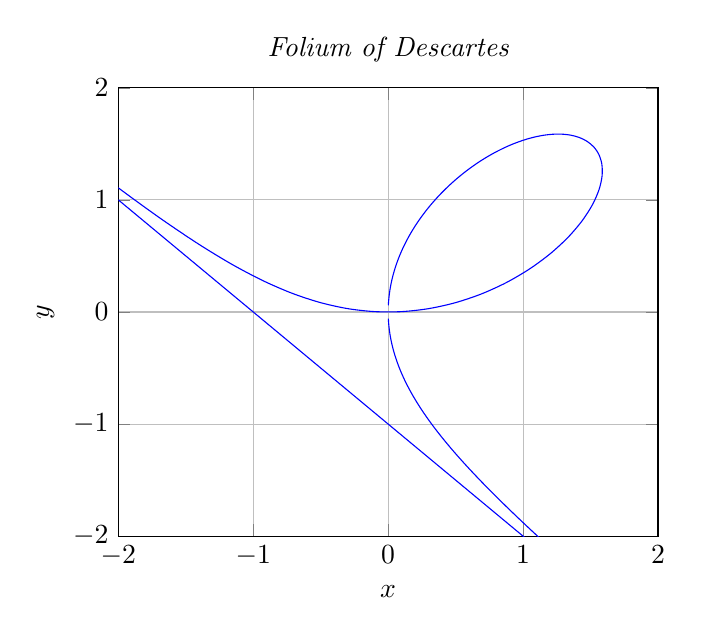
\begin{tikzpicture}
		\begin{axis}[
			title={\it  Folium of Descartes},
			xmin=-2,xmax=2,
			ymin=-2,ymax=2,
			xlabel={$x$},
			ylabel={$y$},
			empty line=jump,
			grid=major,
			]
			\addplot [
			blue,
			domain=-50:50,samples=1500,smooth]
			({3*x/(1+x^3)},{3*x^2/(1+x^3)});
		\end{axis}
	\end{tikzpicture}
\end{center}
\item[v)]
	This follows from calculation that 
	\eq{
	\left(\ff{3t}{1+t^3}\right)^3+\left(\ff{3t^2}{1+t^3}\right)^3
	=27\left(\ff{1}{1+t^3}\right)^3 t^3(1+t^3)=3\ff{3t}{1+t^3}\ff{3t^2}{1+t^3}
	}
	namely $(x,y)$ on the curve only if
	\eq{
	x^3+y^3=3xy
	}
	for the if part, we set $t:=y/x$ when $x\neq0$ and compute that
	\eq{
	&\ff{3t}{1+t^3}=\ff{3x^2y}{x^3+y^3}=\ff{3x^2y}{3xy}=x\\
	&\ff{3t^2}{1+t^3}=\ff{3y^2x}{x^3+y^3}=\ff{3x^2y}{3xy}=y
	}
	thus $(x,y)$ on the curve $x^2+y^3=3xy$ implies that there exist $t$ such that
	$x={3t}/{(1+t^3)}$, $y={3t^2}/{(1+t^3)}$. And for $(0,0)$ we set $t=0$.\\
	This completes the proof.\qed
}
\end{document}
